\chapter{Company description}
\section{Organizational chart}
Through previous endevors, research and talks with various people which work in different management positions, we've come to this organizational chart. The diagram \ref{fig:organisational-chart} depicts all required departments and their teams as well as management positions. Division are marked with the same color. The color's saturation denotes the hirachical position within said department.

\begin{figure}[!ht]
  \centering
  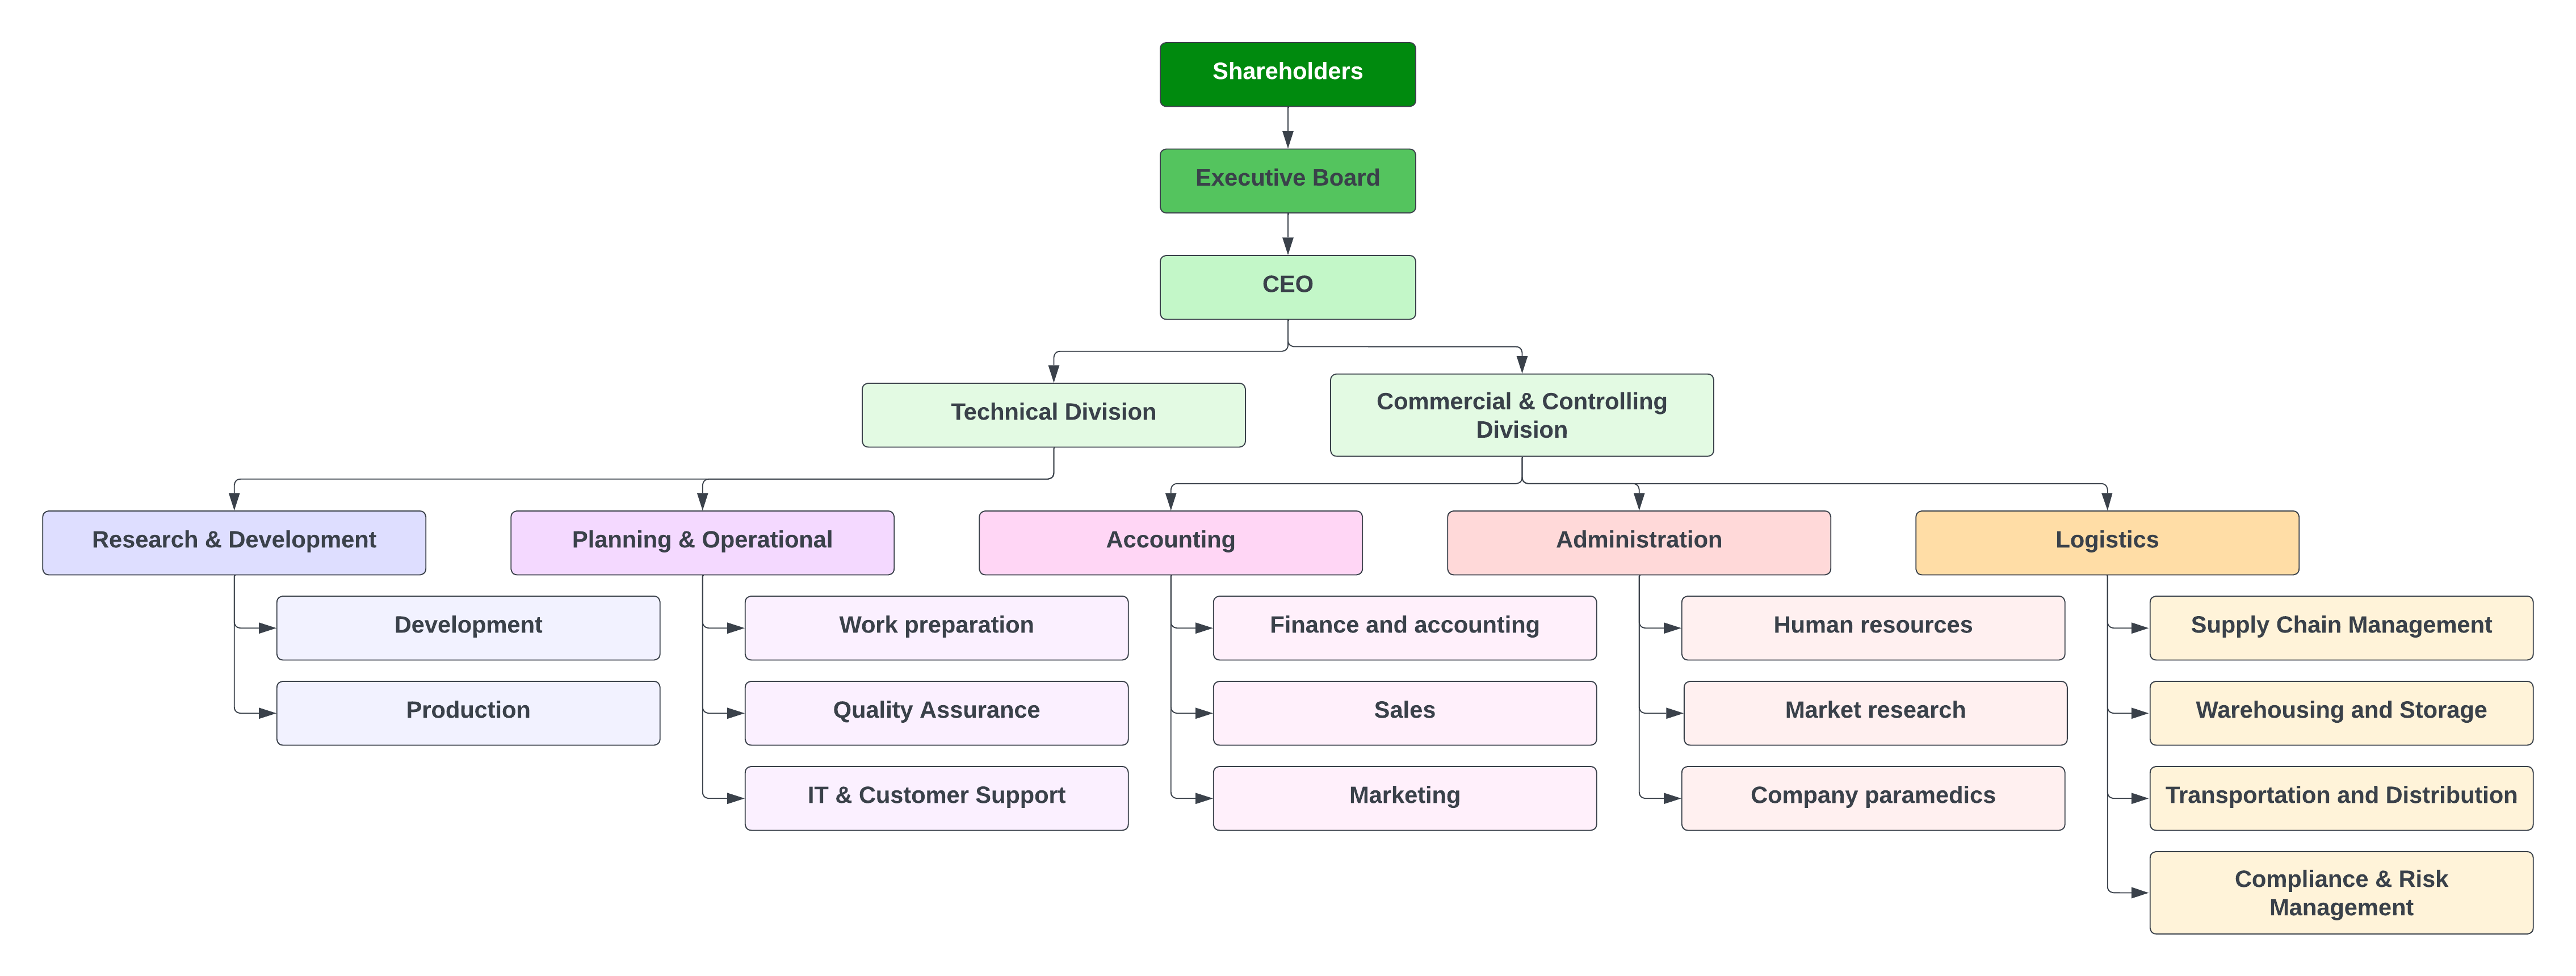
\includegraphics[width=\linewidth]{./images/organisational-chart.png}
  \caption[Organizational chart made with lucidchart.com]{Diagram of the organization}
  \label{fig:organisational-chart}
\end{figure}

This diagram might be more detailed or complex when compared to ones from different startups, but this is by design. It is important that our service works reliably and follows industry standards. To achieve that, we structurally trade a bit of agility for reliability and structure.

Not displayed are ways or means of communication between teams and/or departments. Also, in the future there might be an additional team, which's job is to ignore department barriers and work on different tasks or enable better communication or a better work flow, depending on the workload of a department.

The following chapters \ref{org-management} through \ref{org-logistics} will now go into further detail on what each department entails and of what teams it is made of.
\subsection{Management}\label{org-management}
The management division is marked with the color green. This diagram also includes the shareholders and the executive board. This was done in order to paint a complete picture about the company and how has a say in key decisions.
\newline
Shareholders want to maximize their profit. Keeping them safe and happy is detrimental to the long term success of the company.
\newline
The executive board's and the CEO's job is to lead the company to success and thus growth and profitability. They, especially the CEO, have the big picture in mind and guide the departments to said goals. He has a say in both the "Technical Division" and the "Commercial \& Controlling Division".
\newline
\newline
If uncertainties arise, consulting is also an option to get an external perspective.
\subsection{Research \& Development}
This department is marked with the color indigo.
\newline
By choice, we've structured this technical department into two teams. Both are concerned with "Research \& Development", but one focuses on software while the other focuses on hardware. It's detrimental to us, that both hard and software is done in-house. Having the software team in-house instead of offshore increases the quality, general understanding and agility of our software. Also having hardware in-house enables these teams to work closely together, which further increases the products (and thus also the services) quality and may also lead to a better work environment, as employees are enabled to innovate and take ownership of their own work. \cite{wang_2022_employee}
\subsection{Planning \& Operational}
The "Planning \& Operational" department, marked with violet, is made of a less specialized workforce, which focuses on supporting other departments, customers or general processes.
\subsection{Accounting}
The accounting department is featured with a fuchsia color. It encapsulates a general sales and a marketing team. These are separated and under the same department by design. Their work may be different, but they need to cooperate with each other frequently, which would be harder if they were in different departments.
Additionally, the "Finance and accounting" team is also under this department. It handles all monetary things.
\subsection{Administration}
The red administration department features a classical "Human resources" team, as well as internal paramedics and the "Market research" team. The last one is concerned with the development of the overall market we operate in and how we maneuver in it. It's findings are detrimental, reported to the CEO, which in turn influences the roadmap of the (TODO: acronym) R\&D department.
\subsection{Logistics}\label{org-logistics}
Lastly the logistics department marked with orange. The decision to produce both soft- and hardware in-house requires a bigger logistical effort than if it was done offshore. One team will overlook the supply chain, so that if a global supply bottleneck occurs, we're going to be the least impacted as possible. Two other teams are concerned with warehousing of material while another looks after transportation of goods.
\section{Vision}
\section{Mission}
\section{Contributions to sustainability}
\section{Objectives of services}
